\documentclass[11pt]{article}
\usepackage{UF_FRED_paper_style}

\usepackage{lipsum}  %% Package to create dummy text (comment or erase before start)
\usepackage{listings}% http://ctan.org/pkg/listings
\lstset{
  basicstyle=\ttfamily,
  mathescape
}
%% ===============================================
%% Setting the line spacing (3 options: only pick one)
% \doublespacing
% \singlespacing
\onehalfspacing
%% ===============================================

\setlength{\droptitle}{-5em} %% Don't touch
% %%%%%%%%%%%%%%%%%%%%%%%%%%%%%%%%%%%%%%%%%%%%%%%%%%%%%%%%%%
% SET THE TITLE
% %%%%%%%%%%%%%%%%%%%%%%%%%%%%%%%%%%%%%%%%%%%%%%%%%%%%%%%%%%

% TITLE:
\title{Integer Factorisation Problem \& Modern Factoring Algorithms}
% \thanks{}


% AUTHORS:
\author{Vishisht Priyadarshi\\ 180123053 \\
    \href{mailto:vishisht@iitg.ac.in}{\texttt{vishisht@iitg.ac.in}} %% Email author 1 
\and Sidharth Bankupalle\\ 180123047 \\
    \href{mailto:bankupal@iitg.ac.in}{\texttt{bankupal@iitg.ac.in}} %% Email author 2
    }


% DATE:
\date{\today}

% %%%%%%%%%%%%%%%%%%%%%%%%%%%%%%%%%%%%%%%%%%%%%%%%%%%%%%%%%%
% %%%%%%%%%%%%%%%%%%%%%%%%%%%%%%%%%%%%%%%%%%%%%%%%%%%%%%%%%%
\begin{document}
% %%%%%%%%%%%%%%%%%%%%%%%%%%%%%%%%%%%%%%%%%%%%%%%%%%%%%%%%%%
% %%%%%%%%%%%%%%%%%%%%%%%%%%%%%%%%%%%%%%%%%%%%%%%%%%%%%%%%%%
% ABSTRACT
% %%%%%%%%%%%%%%%%%%%%%%%%%%%%%%%%%%%%%%%%%%%%%%%%%%%%%%%%%%
% %%%%%%%%%%%%%%%%%%%%%%%%%%%%%%%%%%%%%%%%%%%%%%%%%%%%%%%%%%
{\setstretch{1.0}
\maketitle
% %%%%%%%%%%%%%%%%%%
\begin{abstract}
    \emph{"The problem of distinguishing prime numbers from composite numbers, and of resolving the latter into their prime factors, is known to be one of the most important and useful in arithmetic.”}
    
    The Integer Factorization problem is defined as follows:
    \textbf{Given a composite integer $N$, find a non-trivial factor e of $N$, i.e. find e such that e divides $N$.}
    
    When the numbers are sufficiently large, no efficient, non-quantum integer factorization algorithm is known.The most straightforward method of factoring is trial division, which, essentially, checks for every prime number $p$, such that $p \leq \sqrt{n}$ , if $p$ divides $N$. However, trial division may take more than $O\left( \sqrt {N}\right) $ bit operations, which makes it extremely inefficient for the numbers of interest.
    
    Currently there is no known algorithm for answering the question "Does integer $n$ have a factor less than integer s?" in a number of steps that is $O\left( P\left( n\right) \right)$, where $n$ is the number of digits in $N$, and $P\left(n\right)$ is a polynomial function. Moreover, no one has proved that such an algorithm exists, or does not exist
    
    In this project, we aim to do an analysis of the modern Factoring Algorithms and their constraints.

% END CONTENT ABS------------------------------------------
\end{abstract}
}

% %%%%%%%%%%%%%%%%%%%%%%%%%%%%%%%%%%%%%%%%%%%%%%%%%%%%%%%%%%
% BODY OF THE DOCUMENT
% %%%%%%%%%%%%%%%%%%%%%%%%%%%%%%%%%%%%%%%%%%%%%%%%%%%%%%%%%%


%%%%%%%%%%%%%%%%%%%%%%%%%%%%%%%%%%%%%%%%%%%%%%%%%%%%%%%%%%%%%%%%%%%%%%
% --------------------
\section*{Introduction}
% --------------------
\begin{flushleft}
    Integer factoring is a well-known number theory problem with wide applications in complexity and cryptography.
    In this project, we will discuss these factoring algorithms in detail - making way through all the intricate details and their time complexity analysis:\break
    1. Fermat's Factorisation Method\break
    2. Pollard's p-1 Factorisation Algorithm\break
    3. Pollard's Rho Algorithm\break
    4. Linear Sieve\break
\end{flushleft}
%%%%%%%%%%%%%%%%%%%%%%%%%%%%%%%%%%%%%%%%%%%%%%%%%%%%%%%%%%%%%%%%%%%%%%



%%%%%%%%%%%%%%%%%%%%%%%%%%%%%%%%%%%%%%%%%%%%%%%%%%%%%%%%%%%%%%%%%%%%%%
% --------------------
\section*{1. Fermat's Factorisation Method}
% --------------------

\begin{flushleft}
    \textbf{\underline{PROBLEM: }}The Fermat's Factorisation method can be applied to arbitrary odd $n$ to find a divisor pair that are relatively close together, if such a pair exists.
    \break\break
    \textbf{\underline{MAIN IDEA: }}\break
        Consider $n$ to be an odd number(without loss of generality). If $n$ has a non-trivial factors, then $n$ can be written as $n = (x+y)(x-y)$ for some numbers $x$, $y$ $\in \mathbb{N}$ s.t. $x+y$, $x-y$ is not equal to $1$ and $n$.\break\break
        To implement this concept, we define a variable $a$ with initial value of $x^{2}-n$ where $x$ is initialised with a value of $\lfloor \sqrt {n}\rfloor $. Now we iterate over a loop until we found that $a$ is a perfect square. We update the value of $x$ over each iteration by adding odd numbers to it in a sequential way, starting from $2x+1$.
        That is, initially $a = x^{2}-n$, then after first iteration it becomes $\left( x+1\right) ^{2}-n$ since $\left( x+1\right) ^{2}=x^{2}+2x+1$. With each iteration, $a$ takes the values $\left( x+1\right) ^{2}-n$, $\left( x+2\right) ^{2}-n$ and so on until loop terminates.
        At the termination of the loop, we would have $a = x'^{2}-n$ where $a$ can be written as $a=y^{2}$. So, we have $n=x'^{2}-y^{2}$ and hence we have successfully factored $n$.
        \break

    \textbf{\underline{ALGORITHM: }}
        \begin{lstlisting}
        $x\leftarrow \lfloor \sqrt {n}\rfloor$ 
        $t\leftarrow 2x+1$
        $a\leftarrow x^{2}-n$
        while($a$ is not a square of some $k \in \mathbb{N})$
        {
            $a\leftarrow a+t$
            $t\leftarrow t+2$
        }
        $x \leftarrow \left( t-1\right) /2$
        $y\leftarrow \sqrt {a}$
        return $x+y$ and $x-y$ as factors of $n$
        \end{lstlisting}
    
    \textbf{\underline{TIME COMPLEXITY: }}\break
        Let the odd composite number $n$ be written as $n=ab$. Then at the termination $a=x-y$ and $b=x+y$. Now to count the number of iterations, we can take help of $t$. Initially, $t$ will begin with $2x+1$. So, roughly $t$ can be considered to be $2\sqrt {n}$ and at the termination $t = 2x+1 = 1+a+b$.\break
        Hence the number of iterations  = $\dfrac {1}{2}\left( 1+a+b-2\sqrt {n}\right) = \dfrac {1}{2}\left( 1+a+\dfrac {n}{a}-2\sqrt {n}\right)\\ \;\;\;\;\;\;\;\;\;\;\;\;\;\;\;\;\;\;\;\;\;\;\;\;\;\;\;\;\;\;\;\;\;\;\;\;\;\;\;\;\;\;\;\;\;\;\;\;\;\;\;=
        \dfrac {1}{2}\left( 1+\dfrac {\left( \sqrt {n}-a\right) ^{2}}{a}\right) $ 
        \break\break
        As it is evident that the algorithm performs poorly than Trial Division in some of the cases. It works well only when $a$ is very close to $\sqrt{
        n}.$


\end{flushleft}
%%%%%%%%%%%%%%%%%%%%%%%%%%%%%%%%%%%%%%%%%%%%%%%%%%%%%%%%%%%%%%%%%%%%%%



%%%%%%%%%%%%%%%%%%%%%%%%%%%%%%%%%%%%%%%%%%%%%%%%%%%%%%%%%%%%%%%%%%%%%%
% --------------------
\section*{2. Pollard’s p-1 Factorisation Algorithm}
\begin{flushleft}
    % --------------------
    \textbf{\underline{PROBLEM: }} Suppose we have a positive integer $n$ such that it can be expressed as product of 2 primes numbers, i.e. $n$ = $pq$, where, $p$ and $q$ are primes.
    Our aim is to find out $p$ and $q$.
    \break \break
    \textbf{\underline{MAIN IDEA: }}\break
        $p$ is prime $\Rightarrow$ $p$ - 1 is composite
        \break
        Let $p-1=a^{i_{1}}_{1}a^{i_{2}}_{2}\ldots a^{i_{k}}_{k}$ \quad \quad ,where $a_{1},a_{2},\ldots ,a_{k}$ are primes.
        \break
        Consider a number $L$ s.t. $L\geq \max \left\{ a^{i_{1}}_{1}, a^{i_{2}}_{2}, \ldots , a^{i_{k}}_{k}\right\} $
        \break
        Now $L$! = $L$.($L$-1).($L$-2)...1 must be divisible by $p$-1, since all prime powers of ($p$-1) exist in the terms of $L$! at least once.
        \break\break
        By Fermat's Little Theorem, for any arbitrary $a$: \quad $a^{p-1}\equiv 1\left( mod \;p\right)$
        \break
        Now since $L!\equiv 0\left(mod\; \left(p-1\right)\right)  \Rightarrow   a^{L!}\equiv 1\left( mod \;p\right) \Rightarrow   a^{L!}-1\equiv 0\left( mod \;p\right)\break \Rightarrow $  p divides $a^{L!}-1$.\break
        $ \therefore \; \gcd \left( a^{L!}-1,n\right) =$ $p$ or $n$
        \break
        We can compute this GCD. If it is not equal to $n$, we have found a prime factor of $n$, i.e., $p$. But if $\gcd \left( a^{L!}-1,n\right) = n  \Rightarrow$ n divides $a^{L!}-1 \Rightarrow$ q divides $a^{L!}-1 \Rightarrow a^{L!}\equiv 1\left( mod \;q\right)$.
        \break
        Now consider $L!=j\left( q-1\right) +k$ \quad , j, k $\in$ $\mathbb{Z}$  and k $\in$ [0, q-1]
        \break
        $\Rightarrow a^{L!}\equiv a^{k}\left( mod \;q\right) \Rightarrow \therefore a^{k}\equiv 1\left( mod \;q\right) $
        \break \break
        \underline{Case (i) k = 0 :} We restart the process with a different random value of a.
        \break
        \underline{Case (ii) k $\neq$ 0 :} $a^{k}\equiv 1\left( mod \;q\right) $ holds true always until a is not divisible by q. But in no way, we can know before-hand if this is the case since p, q are unknown to us. So the best possible way is to restart the process with a random value of a.
        \break \break
    \textbf{\underline{ALGORITHM: }}
        \begin{lstlisting}
            a $\leftarrow$ random()
            for j $\leftarrow$ 2 to BOUND(B)
            {
                a $\leftarrow$ a^j mod n
                d $\leftarrow$ gcd(a-1, n)
                if(1 < d < n)
                    return d
                else if(d = n)
                    RESTART ALGORITHM WITH A NEW VALUE OF a
            }
        \end{lstlisting}
    
    \textbf{\underline{TERMINATION: }}
        \break
        As we compute $a^{L!}$, and take gcd we have two cases:\break
        \underline{Case (i): } If d $>$ 1, we found the gcd and loop terminates.\break
        \underline{Case (ii): } If d = n, we go back and restart the algorithm with a new random value of $a$. It is guaranteed that we will run into some value of $a$ which is multiple of one of the prime factors of $n$. In that case, gcd($a$, $n$) $>$ 1. Say, $p$ divides $a$, and $p$ also divides $a^{L!}-1$
        $\Rightarrow \gcd \left( a^{L!}-1, \;n\right) = p$ . Hence the algorithm terminates.
        
        
        \break\break
        \textbf{\underline{TIME COMPLEXITY: }}
        \break
        Lets discuss time complexity for a single iteration with a fixed value of $a$.\break
        There are $O\left( B\right)$ modular exponentiations, and each requiring $O\left(log B\right)$ multiplications. GCD can be computed in O(log n) time.
        \break
        $ \therefore$ Time Complexity $= O(B. log B. log n + log n) $
\end{flushleft}
%%%%%%%%%%%%%%%%%%%%%%%%%%%%%%%%%%%%%%%%%%%%%%%%%%%%%%%%%%%%%%%%%%%%%%


%%%%%%%%%%%%%%%%%%%%%%%%%%%%%%%%%%%%%%%%%%%%%%%%%%%%%%%%%%%%%%%%%%%%%%
% --------------------
\section*{3. Pollard's Rho Algorithm}
    \begin{flushleft}
    % --------------------
    \textbf{\underline{PROBLEM: }} Suppose we have a positive integer $n$ such that it can be expressed as product of 2 primes numbers, i.e. $n$ = $pq$, where, $p$ and $q$ are primes.
    Our aim is to find out $p$ and $q$.
    \break \break
    \textbf{\underline{MAIN IDEA: }}\break
        Pollard's rho algorithm iterates a simple polynomial map (which should not be a permutation polynomial) and produces a non-trivial divisor of $n$. The map generates a pseudo-random sequence of numbers. \break
        Pollard's rho algorithm uses an iteration of the form:\quad \quad
        $x_{i+1}=f\left( x_{i}\right) mod \; n$ \quad , $i \neq$ 0   
        where $n$ is the number to be factored, $x_{0}$ is a random starting value and $f$ is a polynomial with integer coefficients.
        In practice, $f\left( x\right) = x^{2}+a$ is chosen ( a $\neq$ 0, -2 since they are fixed points for $f\left( x\right) $ ). \break \break
        Now the algorithm proceeds as follows: \break
        \underline{STEP 1. :} Compute $d = gcd\left( x-x',n\right) ,\;\; x'=f\left( x\right) $ \break
        \underline{STEP 2. :} If $1 < d < n$, $d$ is a proper divisor of $n$.
         \break \quad If d = 1, replace $x$ by $f\left( x\right)$, and $x'$ by $f\left(f\left( x'\right)\right)$ \break
        If d = n, algorithm has to be re-initialised, since we encountered a failure.
         \break \break
        In short, we are looking for two distinct values $x_{i},x_{j}\in \mathbb{Z} _{n}$ s.t. $gcd\left( x_{i}-x_{j},n\right)  >1$. This is reasoned out by the fact that if $gcd\left( x_{i}-x_{j},n\right)  >1 \Rightarrow \; gcd\left( x_{i}-x_{j},n\right)$ is a factor of $n$, which is either $p$ or $q$.\\
        But whether we will get $gcd\left( x_{i}-x_{j},n\right)  >1$ and that too in reasonable number of steps is answered by the Birthday Paradox. In fact, Pollard's Rho Algorithm can be seen as a re-formulation of Birthday Paradox Problem, which we will discuss now: \break \break
        Now say we pick $k$ numbers $x_{1},x_{2},\ldots ,x_{k}$ uniformly at random in  $\mathbb{Z} _{n}$. Suppose that these $k$ numbers are distinct. Now let's say that there exists some $1\neq i < j \neq k$ s.t. $x_{i}=x_{j}\left( mod\:p\right) $. Then $p\;|\;x_{i}-x_{j}$, and since $p\;|\;n$ also , we have $p\;|\;gcd\left( x_{i}-x_{j},n\right)$. \break
        Moreover since $x_{i}, x_{j} \in \mathbb{Z}_{n}$ and they are distinct $\Rightarrow gcd\left( x_{i}-x_{j},n\right) < n \Rightarrow \; \therefore gcd\left( x_{i}-x_{j},n\right)$ provides a non-trivial factor of $n$. \break
        But we need to find an upper-bound on size of k such that it is guaranteed that if we compute $gcd\left( x_{i}-x_{j},n\right)$ for all pairs of $1 \leq i < j \leq k$, we find a non-trivial factor. \break
        Now, 
        \begin{equation}
          \label{q-def}
         x_{i}\equiv x_{j}\left( mod \; p\right)
        \end{equation}
        Lets calculate the probability that equation~\eqref{q-def} does not hold, i.e., $\left( x_{1},x_{2},\ldots ,x_{k}\right) mod \; p $ are all different.
        \begin{equation}
        \mathbb{P} = \left( 1-\dfrac {1}{n}\right) \left( 1-\dfrac {2}{n}\right) \ldots \left( 1-\dfrac {k-1}{n}\right) 
        \leq e^{-\dfrac {1}{n}}.e^{-\dfrac {2}{n}}\ldots e^{-\dfrac {k-1}{n}}=e^{\dfrac {-k\left( k-1\right) }{2n}} \sim e^{\dfrac {-k^{2}}{2n}}
        \end{equation}
        Since $p \leq \sqrt{n}$, $k = n^{\dfrac {1}{4}}$ is suitable since it gives a higher probability that (1) holds\\
        Now we use the pseudo-random generator function to generate the k numbers in sequence and search for the pair i, j s.t. $i < j$ and $x_{i} \equiv x_{j} \left( mod \; p \right). $ But checking all the $\begin{pmatrix}
        k \\ 2 \end{pmatrix}$ pairs will result in a lot of GCD computations, thereby resulting in time complexity which is of the order $\sqrt {n}$. \break \break
        An optimisation that we can make here is to reduce the number of GCD computations by using Floyd's Cycle Detection Algorithm. We can easily show that: $x_{i} \equiv x_{j} \left( mod \; p \right) \rightarrow x_{i+1} \equiv x_{j+1} \left( mod \; p \right)$ which we can generalise as: $x_{i+\delta} \equiv x_{j+\delta} \left( mod \; p \right) \forall \; \; \delta \req 0 $.\break Eventually the sequence runs into a cycle. So our task reduces to finding  $x_{i} \equiv x_{j} \left( mod \; p \right)$ with $i < j$ and i as small as possible. \break
        Now it is an established fact that there will be a pair $i < j < C_{o}\sqrt{p}$ \quad ($C_{o}$ is a constant) s.t. $x_{i} \equiv x_{j} \left( mod \; p \right)$ (based on empirical calculations). So our algorithm finds out the factor of $n$ in $O\left( n^{1/4}\right)$ time.
      \break \break
     \textbf{\underline{ALGORITHM: }}
        \begin{lstlisting}
            INITIALISE POLYNOMIAL MAP $f$
            $x \leftarrow x_{o}$
            $x' \leftarrow f\left( x\right) \left( mod \; n\right) $
            $p \leftarrow$ gcd($x - x', n$)
            while($p$ = 1)
            {
                $x \leftarrow x_{i}$
                $x' \leftarrow x_{2i}$
                $x \leftarrow f\left( x\right) \left( mod \; n\right) $
                $x' \leftarrow f\left( x'\right) \left( mod \; n\right) $
                $x'  \leftarrow f\left( x'\right) \left( mod \; n\right) $
                $p \leftarrow $ gcd($x - x', n$)
            }
            if($p$ = $n$)
                return "$n$ is prime"
            else
                return $p$
        \end{lstlisting}
    \textbf{\underline{TIME COMPLEXITY: }}\break
        As discussed in the previous section, the Pollard's Rho algorithm is able to find a factor $p$ of $n$ with an expected number of $\Theta \left( \sqrt {p}\right) $ of arithmetic operations, that is, about an order of $\Theta \left( n^{1/4}\right) $.

\end{flushleft}
%%%%%%%%%%%%%%%%%%%%%%%%%%%%%%%%%%%%%%%%%%%%%%%%%%%%%%%%%%%%%%%%%%%%%%



%%%%%%%%%%%%%%%%%%%%%%%%%%%%%%%%%%%%%%%%%%%%%%%%%%%%%%%%%%%%%%%%%%%%%%
% --------------------
\section*{4. Linear Sieve}
% --------------------
\begin{flushleft}
    \textbf{\underline{PROBLEM: }}Given a number n, find all prime numbers in a segment $\left[ 2,n\right]$ in linear time complexity
    \break\break
    \textbf{\underline{MAIN IDEA: }}\break
        The sieve of Eratosthenes is probably the simplest way to pick out all the primes in a given range from $2$ to $n$ but it has time complexity $O\left( n\log \log n\right) $. The algorithm described below is interesting by its simplicity: it isn't any more complex than the classic sieve of Eratosthenes but has linear complexity.\break
        Our goal is to calculate minimum prime factor $lp\left[ i\right] $ for every number $i$ in the segment $\left[ 2,n\right]$. Besides, we need to store the list of all the found prime numbers - let's call it $pr\left[ \right] $.
        We'll initialize the values $lp\left[ i\right]$ with zeros, which means that we assume all numbers are prime. During the algorithm execution this array will be filled gradually. Now we'll go through the numbers from $2$ to $n$. We have two cases for the current number $i$:\break\break
        \underline{Case 1 : $lp\left[ i\right]=0$ -} This means that i is prime, i.e. we haven't found any smaller factors for it. Hence, we assign $lp\left[ i\right]=i$ and add $i$ to the end of the list $pr\left[ \right] $.\break
        \underline{Case 1 : $lp\left[ i\right]\neq 0$ -} This means that $i$ is composite, and its minimum prime factor is $lp\left[ i\right]$.\break\break
        In both cases we update values of $lp\left[\right]$ for the numbers that are divisible by $i$. However, our goal is to learn to do so as to set a value $lp\left[\right]$ at most once for every number. We can do it as follows:\break
        
        Let's consider numbers $x_{j}=i\cdot p_{j}$, where $ p_{j}$ are all prime numbers less than or equal to $lp\left[ i\right]$ (this is why we need to store the list of all prime numbers).\break
        We'll set a new value $lp\left[ x_{j}\right] =p_{j}$ for all numbers of this form.
        \break\break
    \textbf{\underline{ALGORITHM: }}
        \begin{lstlisting}
        Enter a natural number n
        Initialise array lp[n]
        Initialise list pr
        for i <- 2 to n
        {
            if(lp[i] = 0)
            {
                lp[i] <- i
                push back i to pr
            }
            for j <- 1 to size(pr)
            {
                if(pr[j] <= lp[i] AND (i*pr[j]) <= n)
                {
                    lp[i*pr[j]] = pr[j]
                }
            }
        }
        return lp[]
        
    \end{lstlisting}
    
    
    \textbf{\underline{TIME \& SPACE COMPLEXITY:}}
    \end{flushleft}
        Although the running time of $O\left( n\right) $ is better than $O\left( n\log \log n\right) $ of the classic sieve of Eratosthenes, the difference between them is not so big. In practice that means just double difference in speed, and the optimized versions of the sieve run as fast as the algorithm given here.
        Considering the memory requirements of this algorithm - an array $lp\left[ \right] $ of length n, and an array of $pr\left[ \right] $ of length $\dfrac {n}{\ln n}$, this algorithm requires 32 times the memory needed for the classic sieve.
        However, its usefulness is that this algorithm calculates an array $lp\left[ \right] $, which allows us to find factorization of any number in the segment $\left[ 2;n\right] $ in the time of the size order of this factorization. Moreover, using just one extra array will allow us to avoid divisions when looking for factorization.
        Knowing the factorizations of all numbers is very useful for some tasks, and this algorithm is one of the few which allow to find them in linear time.
%%%%%%%%%%%%%%%%%%%%%%%%%%%%%%%%%%%%%%%%%%%%%%%%%%%%%%%%%%%%%%%%%%%%%%



%%%%%%%%%%%%%%%%%%%%%%%%%%%%%%%%%%%%%%%%%%%%%%%%%%%%%%%%%%%%%%%%%%%%%%
% --------------------
% --------------------
\section*{Conclusion}
\begin{flushleft}
% --------------------
% --------------------
    We are interested in factoring, because it is an example of an algorithmic problem on which there has been well-documented progress. As well as their inherent interest and applicability to other areas of mathematics, advances in public key cryptography have lent algorithms for integer factorisation a lot of practical importance. Despite much progress in the development of efficient algorithms, our knowledge of the complexity of factorisation is inadequate. We would like to find a polynomial time factorisation algorithm or else prove that one does not exist. Until a polynomial time algorithm is found or a quantum computer capable of running Shor's algorithm(a polynomial time quantum computer algorithm) is built, large factorisations will remain an interesting challenge.
    \break \break
    The general number field sieve (GNFS) is the most efficient classical algorithm known for factoring integers larger than $10^{100}$. It is a randomized algorithm and heuristically, we get an expected complexity of $O\Big(e^{\sqrt{\frac{64}{9}}(\log N)^{\frac 13}(\log\log N)^{\frac 23}}\Big)$.\break
    GNFS has been to able factor numbers up to 576 bits long. However, it seems quite improbable that a PC-based implementation of the algorithm can do much better. That is why, other, non-algorithmic methods, have been proposed to improve the efficiency of the existing algorithms.\break \break
    Some of these includes ideas of Distributed Computing, use of special hardwares(like Sieve Devices) and use of Quantum Computers (Shor's Algorithm). 
    \end{flushleft}

%

\begin{figure}[H]
    \centering
        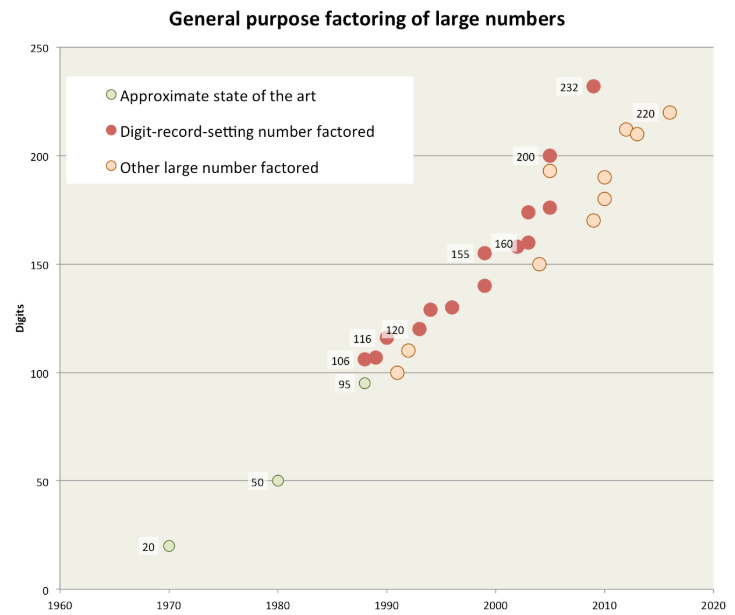
\includegraphics[scale=.6]{figures/GPR - 2.png}
    \caption{Figure 1: Size of numbers (in decimal digits) that could be factored over recent history. Green ‘approximate state of the art’ points do not necessarily represent specific numbers or the very largest that could be at that time—they are qualitative estimates. The other points represent specific large numbers being factored, either as the first number of that size ever to be factored (red) or not (orange). Dates are accurate to the year. Some points are annotated with decimal digit size, for ease of reading.
}

    \label{fig:1}
\end{figure}
%%%%%%%%%%%%%%%%%%%%%%%%%%%%%%%%%%%%%%%%%%%%%%%%%%%%%%%%%%%%%%%%%%%%%%


%%%%%%%%%%%%%%%%%%%%%%%%%%%%%%%%%%%%%%%%%%%%%%%%%%%%%%%%%%%%%%%%%%%%%%
% --------------------
% --------------------
\section*{References}
% --------------------
% --------------------
\begin{enumerate}
\itemsep-0.5em
    \item Arjen K. Lenstra, \emph{General purpose integer factoring}
    \item Kostas Bimpikis and Ragesh Jaiswal, \emph{Modern Factoring Algorithms}
    \item Richard P. Brent, \emph{An improved Monte Carlo Factorization Algorithm}, $\left( 1980\right)$ 
    \item Peter L. Montgomery, \emph{Speeding the Pollard and Elliptic Curve Methods of Factorization}, \emph{Mathematics of Computation,} Volume 48, Issue 177 (Jan.,1987), 243-264
    \item Eric Bach ,\emph{Toward a Theory of Pollard's Rho Method}, $\left( 1991\right)$
    \item David Gries \& Jayadev Misra, \emph{A Linear Sieve
Algorithm for Finding Prime Numbers }
    \item Anne-Sophie Charest, \emph{Pollard’s p-1 and Lenstra’s factoring
    algorithms}, $\left( 2005\right)$
    \item Sounak Gupta and Goutam Paul, \emph{Revisiting Fermat’s Factorization
    for the RSA Modulus} $\left( 2009\right)$
    \item Robert Erra and Christophe Grenier, \emph{The Fermat factorization method revisited}, $\left( 3oth June 2009\right)$
    \item Soud K. Mohamed, \emph{Analysis of Pollard's Rho Factoring Method}, $\left( 2019\right)$
    \item Samuel S. Wagstaff, Jr., \emph{The Joy of Factoring}, Student mathematical library Volume 68, \emph{Pg - 119 to 142} 
    \item Cristina-Loredana Duta et al., \emph{Framework for evaluation and comparison of integer factorization algorithms}, 2016 SAI Computing Conference $\left( 2016\right)$
\end{enumerate}
%%%%%%%%%%%%%%%%%%%%%%%%%%%%%%%%%%%%%%%%%%%%%%%%%%%%%%%%%%%%%%%%%%%%%%



\end{document}